         \chapter{Functions}
    \setcounter{figure}{1}
    \setcounter{subfigure}{1}
    \label{acabd86c2f495c693bc00f7e5c26834f}
%     
%        
%          \section{ Introduction and key concepts}
%     \nopagebreak
%             \label{m39337} $ \hspace{-5pt}\begin{array}{cccccccccccc}   
\includegraphics[width=0.75cm]{col11306.imgs/summary_fullmarks.png} &   \end{array} $ \hspace{2 pt}\raisebox{-5 pt}{} {(section shortcode: MG10015 )} \par 
%     
%     
%     
%     \label{m39337*cid2}
%             \section{ Introduction to Functions and Graphs}
%             \nopagebreak
      \label{m39337*id231690}Functions are mathematical building blocks for designing machines, predicting natural disasters, curing diseases, understanding world economies and for keeping aeroplanes in the air. Functions can take input from many variables, but always give the same answer, unique to that function. It is the fact that you always get the same answer from a set of inputs that makes functions special.\par 
      \label{m39337*id231697}A major advantage of functions is that they allow us to \textsl{visualise} equations in terms of a \textsl{graph}. A graph is an accurate drawing of a function and is much easier to read than lists of numbers. In this chapter we will learn how to understand and create real valued functions, how to read graphs and how to draw them.\par 
      \label{m39337*id232051}In addition to their use in the problems facing humanity, functions also appear on a day-to-day level, so they are worth learning about. A function is always \textsl{dependent} on one or more variables, like time, distance or a more abstract quantity.\par 
    \label{m39337*cid3}
            \section{ Functions in the Real-World}
            \nopagebreak
 \label{m39337*id232071}Some typical examples of functions you may already have met
include:-\par 
      \label{m39337*id232074}\begin{itemize}[noitemsep]
            \label{m39337*uid1}\item how much money you have, as a function of time. You never have more than one amount of money at any time because you can always add everything to give one number. By understanding how your money changes over time, you can plan to spend your money sensibly. Businesses find it very useful to \textsl{plot the graph} of their money over time so that they can see when they are spending too much. Such observations are not always obvious from looking at the numbers alone.
\label{m39337*uid2}\item the temperature is a very complicated function because it has so many inputs, including; the time of day, the season, the amount of clouds in the sky, the strength of the wind, where you are and many more. But the important thing is that there is only one temperature when you measure it in a specific place. By understanding how the temperature is effected by these things, you can plan
for the day.
\label{m39337*uid3}\item where you are is a function of time, because you cannot be in two places at once! If you were to \textsl{plot the graphs} of where two people are as a function of time, if the lines cross it means that the two people meet each other at that time. This idea is used in \textsl{logistics}, an area of mathematics that tries to plan where people and items are for businesses.
\label{m39337*uid4}\item your weight is a function of how much you eat and how much exercise you do, but everybody has a different function so that is why people are all different sizes.
\end{itemize}
    \label{m39337*cid4}
            \section{ Basic Functions}
            \nopagebreak
      \label{m39337*id235621}There are many characteristics of graphs that help describe the graph of any function. These properties will be described in this chapter and are:\par 
      \label{m39337*id235628}\begin{enumerate}[noitemsep, label=\textbf{\arabic*}. ] 
            \label{m39337*uid31}\item dependent and independent variables
\label{m39337*uid32}\item domain and range
\label{m39337*uid33}\item intercepts with axes
\label{m39337*uid34}\item turning points
\label{m39337*uid35}\item asymptotes
\label{m39337*uid36}\item lines of symmetry
\label{m39337*uid37}\item intervals on which the function increases/decreases
\label{m39337*uid38}\item continuous nature of the function
\end{enumerate}
      \label{m39337*id235730}Some of these words may be unfamiliar to you, but each will be clearly described. Examples of these properties are shown in Figure~1.3.\par 
    \setcounter{subfigure}{0}
	\begin{figure}[H] % horizontal\label{m39337*uid39}
    \begin{center}
    \rule[.1in]{\figurerulewidth}{.005in} \\
        \label{m39337*uid39!!!underscore!!!media}\label{m39337*uid39!!!underscore!!!printimage}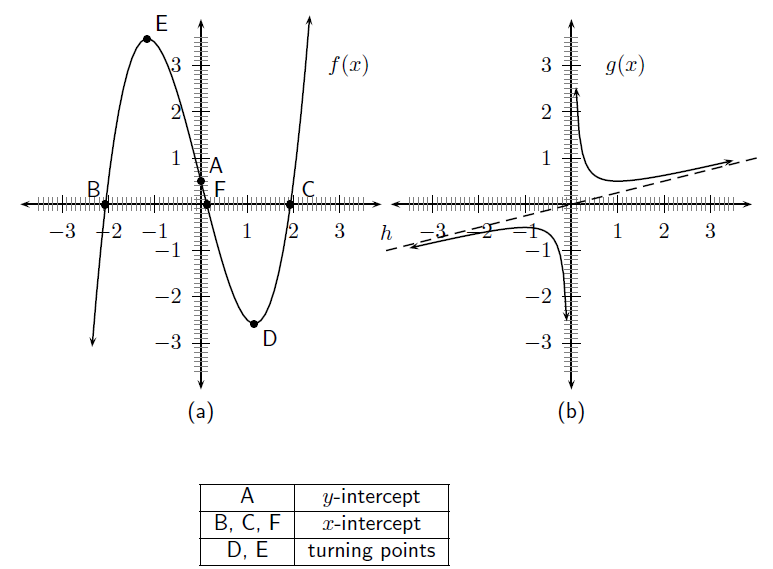
\includegraphics[width=300px]{col11306.imgs/m39337_MG10C11_034.png} % m39337;MG10C11\_034.png;;;6.0;8.5;
      \vspace{2pt}
    \vspace{\rubberspace}\par \begin{cnxcaption}
	  \small \textbf{Figure 1.3: }(a) Example graphs showing the characteristics of a function. (b) Example graph showing asymptotes of a function. The asymptotes are shown as dashed lines.
	\end{cnxcaption}
    \vspace{.1in}
    \rule[.1in]{\figurerulewidth}{.005in} \\
    \end{center}
 \end{figure}       
      \label{m39337*uid40}
            \subsection{ Dependent and Independent Variables}
            \nopagebreak
        \label{m39337*id235764}Thus far, all the graphs you have drawn have needed two values, an $x$-value and a $y$-value. The $y$-value is usually determined from some relation based on a given or chosen $x$-value. These values are given special names in mathematics. The given or chosen $x$-value is known as the \textsl{independent} variable, because its value can be chosen freely. The calculated $y$-value is known as the \textsl{dependent} variable, because its value depends on the chosen $x$-value.\par 
      \label{m39337*uid41}
            \subsection{ Domain and Range}
            \nopagebreak
        \label{m39337*id235855}The \textsl{domain} of a relation is the set of all the $x$ values for which there exists at least one $y$ value according to that relation. The \textsl{range} is the set of all the $y$ values, which can be obtained using at least one $x$ value.\par 
        \label{m39337*id235908}If the relation is of height to people, then the domain is all living people, while the range would be about 0,1 to 3 metres --- no living person can have a height of 0m, and while strictly it's not impossible to be taller than 3 metres, no one alive is. An important aspect of this range is that it does not contain \textsl{all} the numbers between 0,1 and 3, but at most six billion of them (as many as there are people).\par 
        \label{m39337*id235939}As another example, suppose $x$ and $y$ are real valued variables, and we have the relation $y={2}^{x}$. Then for \textsl{any} value of $x$, there is a value of $y$, so the domain of this relation is the whole set of real numbers. However, we know that no matter what value of $x$ we choose, ${2}^{x}$ can never be less than or equal to 0. Hence the range of this function is all the real numbers strictly greater than zero.\par 
        \label{m39337*id236030}These are two ways of writing the domain and range of a function, \textsl{set notation} and \textsl{interval notation}. Both notations are used in mathematics, so you should be familiar with each.\par 
        \label{m39337*uid42}
            \subsection{ Set Notation}
            \nopagebreak
          \label{m39337*id236056}A set of certain $x$ values has the following form:\par 
          \label{m39337*uid43}\nopagebreak\noindent{}
            
    \begin{equation}
    x:\mathrm{conditions,\; more\; conditions}\tag{1.5}
      \end{equation}
          \label{m39337*id236100}We read this notation as ``the set of all $x$ values where all the conditions are satisfied''. For example, the set of all positive real numbers can be written as $\{x:x\in \mathbb{R},x\greatthan{}0\}$ which reads as ``the set of all $x$ values where $x$ is a real number and is greater than zero''.\par 
        \label{m39337*uid44}
            \subsection{ Interval Notation}
            \nopagebreak
          \label{m39337*id236181}Here we write an interval in the form '\textsl{lower bracket, lower number, comma, upper number, upper bracket}'. We can use two types of brackets, square ones $\left[;\right]$ or round ones $\left(;\right)$. A square bracket means including the number at the end of the interval whereas a round bracket means excluding the number at the end of the interval. It is important to note that this notation can only be used for all real numbers in an interval. It cannot be used to describe integers in an interval or rational numbers in an interval.\par 
          \label{m39337*id236225}So if $x$ is a real number greater than 2 and less than or equal to 8, then $x$ is any number in the interval\par 
          \label{m39337*uid45}\nopagebreak\noindent{}
    \begin{equation}
    \left(2;8\right]\tag{1.6}
      \end{equation}
          \label{m39337*id236274}It is obvious that 2 is the lower number and 8 the upper number. The round bracket means 'excluding 2', since $x$ is greater than 2, and the square bracket means 'including 8' as $x$ is less than or equal to 8.\par 
      \label{m39337*uid46}
            \subsection{ Intercepts with the Axes}
            \nopagebreak
        \label{m39337*id236308}The \textsl{intercept} is the point at which a graph intersects an axis. The $x$-intercepts are the points at which the graph cuts the $x$-axis and the $y$-intercepts are the points at which the graph cuts the $y$-axis.\par 
        \label{m39337*id236356}In Figure~1.3(a), the A is the $y$-intercept and B, C and F are $x$-intercepts.\par 
        \label{m39337*id236384}You \textbf{will} usually need to calculate the intercepts. The two most important things to remember is that at the $x$-intercept, $y=0$ and at the $y$-intercept, $x=0$.\par 
        \label{m39337*id236442}For example, calculate the intercepts of $y=3x+5$. For the $y$-intercept, $x=0$. Therefore the $y$-intercept is ${y}_{int}=3\left(0\right)+5=5$. For the $x$-intercept, $y=0$. Therefore the $x$-intercept is found from $0=3{x}_{int}+5$, giving ${x}_{int}=-\frac{5}{3}$.\par 
      \label{m39337*uid47}
            \subsection{ Turning Points}
            \nopagebreak
        \label{m39337*id236645}Turning points only occur for graphs of functions whose highest power is greater than 1. For example, graphs of the following functions will have turning points.\par 
        \label{m39337*id236652}\nopagebreak\noindent{}
          
    \begin{equation}
    \begin{array}{ccc}\hfill f\left(x\right)& =& 2{x}^{2}-2\hfill \\ \hfill g\left(x\right)& =& {x}^{3}-2{x}^{2}+x-2\hfill \\ \hfill h\left(x\right)& =& \frac{2}{3}{x}^{4}-2\hfill \end{array}\tag{1.7}
      \end{equation}
        \label{m39337*id236788}There are two types of turning points: a minimal turning point and a maximal turning point. A minimal turning point is a point on the graph where the graph stops decreasing in value and starts increasing in value and a maximal turning point is a point on the graph where the graph stops increasing in value and starts decreasing. These are shown in Figure~1.4.\par 
    \setcounter{subfigure}{0}
	\begin{figure}[H] % horizontal\label{m39337*uid48}
    \begin{center}
    \rule[.1in]{\figurerulewidth}{.005in} \\
        \label{m39337*uid48!!!underscore!!!media}\label{m39337*uid48!!!underscore!!!printimage}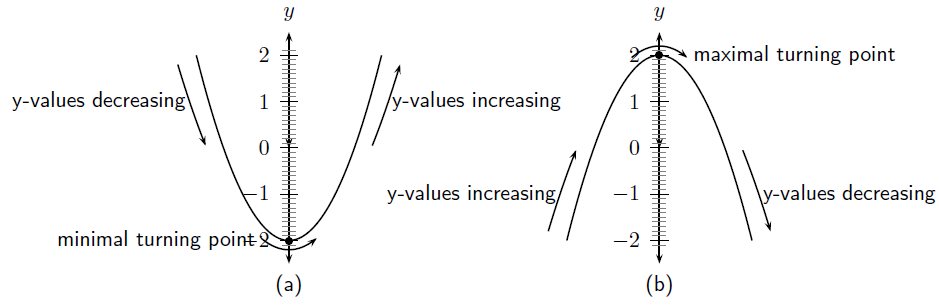
\includegraphics[width=300px]{col11306.imgs/m39337_MG10C11_035.png} % m39337;MG10C11\_035.png;;;6.0;8.5;
      \vspace{2pt}
    \vspace{\rubberspace}\par \begin{cnxcaption}
	  \small \textbf{Figure 1.4: }(a) Maximal turning point. (b) Minimal turning point.
	\end{cnxcaption}
    \vspace{.1in}
    \rule[.1in]{\figurerulewidth}{.005in} \\
    \end{center}
 \end{figure}       
        \label{m39337*id236816}In Figure~1.3(a), E is a maximal turning point and D is a minimal turning point.\par 
      \label{m39337*uid49}
            \subsection{ Asymptotes}
            \nopagebreak
        \label{m39337*id236837}An asymptote is a straight or curved line, which the graph of a function will approach, but never touch.\par 
        \label{m39337*id236844}In Figure~1.3(b), the $y$-axis and line $h$ are both asymptotes as the graph approaches both these lines, but never touches them.\par 
      \label{m39337*uid50}
            \subsection{ Lines of Symmetry}
            \nopagebreak
        \label{m39337*id236883}Graphs look the same on either side of lines of symmetry. These lines may include the $x$- and $y$- axes. For example, in Figure~1.5 is symmetric about the $y$-axis. This is described as the axis of symmetry. Not every graph will have a line of symmetry.\par 
    \setcounter{subfigure}{0}
	\begin{figure}[H] % horizontal\label{m39337*uid51}
    \begin{center}
    \rule[.1in]{\figurerulewidth}{.005in} \\
        \label{m39337*uid51!!!underscore!!!media}\label{m39337*uid51!!!underscore!!!printimage}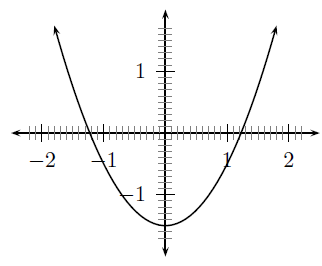
\includegraphics[width=300px]{col11306.imgs/m39337_MG10C11_036.png} % m39337;MG10C11\_036.png;;;6.0;8.5;
      \vspace{2pt}
    \vspace{\rubberspace}\par \begin{cnxcaption}
	  \small \textbf{Figure 1.5: }Demonstration of axis of symmetry. The $y$-axis is an axis of symmetry, because the graph looks the same on both sides of the $y$-axis.
	\end{cnxcaption}
    \vspace{.1in}
    \rule[.1in]{\figurerulewidth}{.005in} \\
    \end{center}
 \end{figure}       
      \label{m39337*uid52}
            \subsection{ Intervals on which the Function Increases/Decreases}
            \nopagebreak
        \label{m39337*id236961}In the discussion of turning points, we saw that the graph of a function can start or stop increasing or decreasing at a turning point. If the graph in Figure~1.3(a) is examined, we find that the values of the graph increase and decrease over different intervals. We see that the graph increases (i.e. that the $y$-values increase) from -$\infty $ to point E, then it decreases (i.e. the $y$-values decrease) from point E to point D and then it increases from point D to +$\infty $.\par 
      \label{m39337*uid53}
            \subsection{ Discrete or Continuous Nature of the Graph}
            \nopagebreak
        \label{m39337*id237022}A graph is said to be continuous if there are no breaks in the graph. For example, the graph in Figure~1.3(a) can be described as a continuous graph, while the graph in Figure~1.3(b) has a break around the asymptotes which means that it is not continuous.
In Figure~1.3(b), it is clear that the graph does have a break in it around the asymptote.\par 
\label{m39337*secfhsst!!!underscore!!!id796}
            \subsection{  Domain and Range }
            \nopagebreak
        \label{m39337*id237058}\begin{enumerate}[noitemsep, label=\textbf{\arabic*}. ] 
            \label{m39337*uid54}\item The domain of the function $f\left(x\right)=2x+5$ is -3; -3; -3; 0. Determine the range of $f$.
        \label{m39337*uid55}\item If $g\left(x\right)=-{x}^{2}+5$ and $x$ is between - 3 and 3, determine:
\label{m39337*id237164}\begin{enumerate}[noitemsep, label=\textbf{\alph*}. ] 
            \label{m39337*uid56}\item the domain of $g\left(x\right)$\label{m39337*uid57}\item the range of $g\left(x\right)$\end{enumerate}
                \label{m39337*uid58}\item On the following graph label:
\label{m39337*id237234}\begin{enumerate}[noitemsep, label=\textbf{\alph*}. ] 
            \label{m39337*uid59}\item the $x$-intercept(s)
\label{m39337*uid60}\item the $y$-intercept(s)
\label{m39337*uid61}\item regions where the graph is increasing
\label{m39337*uid62}\item regions where the graph is decreasing
\end{enumerate}
    \setcounter{subfigure}{0}
	\begin{figure}[H] % horizontal\label{m39337*id237308}
    \begin{center}
    \label{m39337*id237308!!!underscore!!!media}\label{m39337*id237308!!!underscore!!!printimage}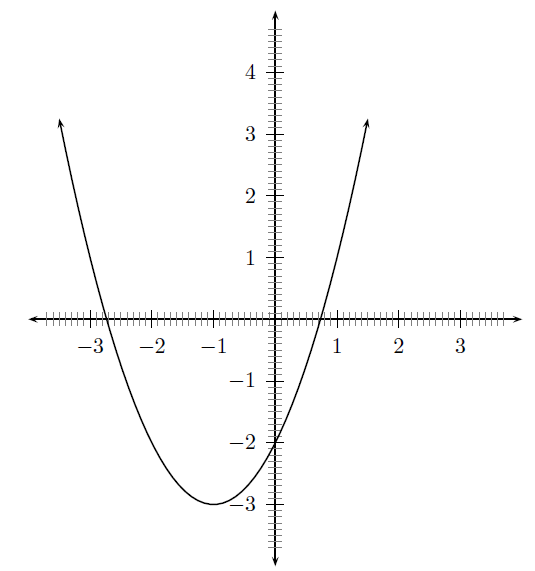
\includegraphics[height=300px]{col11306.imgs/m39337_MG10C11_003.png} % m39337;MG10C11\_003.png;;;6.0;8.5;
      \vspace{2pt}
    \vspace{.1in}
    \end{center}
 \end{figure}               \label{m39337*uid63}\item On the following graph label:
\label{m39337*id237327}\begin{enumerate}[noitemsep, label=\textbf{\alph*}. ] 
            \label{m39337*uid64}\item the $x$-intercept(s)
\label{m39337*uid65}\item the $y$-intercept(s)
\label{m39337*uid66}\item regions where the graph is increasing
\label{m39337*uid67}\item regions where the graph is decreasing
\end{enumerate}
    \setcounter{subfigure}{0}
	\begin{figure}[H] % horizontal\label{m39337*id237401}
    \begin{center}
    \label{m39337*id237401!!!underscore!!!media}\label{m39337*id237401!!!underscore!!!printimage}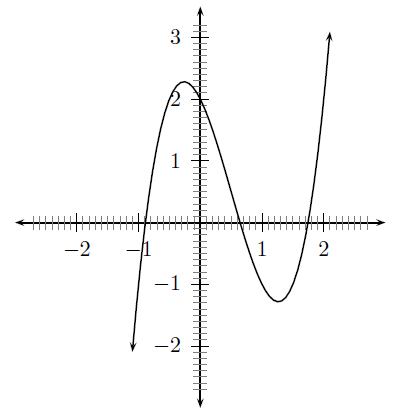
\includegraphics[height=300px]{col11306.imgs/m39337_MG10C11_004.png} % m39337;MG10C11\_004.png;;;6.0;8.5;
      \vspace{2pt}
    \vspace{.1in}
    \end{center}
 \end{figure}               \end{enumerate}
\label{m39337**end}
\par \raisebox{-5 pt}{
\includegraphics[width=0.5cm]{col11306.imgs/summary_www.png}} Find the answers with the shortcodes:
 \par \begin{tabular}[h]{cccccc}
 (1.) lxY  &  (2.) lxg  &  (3.) lx4  &  (4.) lx2  & \end{tabular}
% 
%          \section{ The straight line}
%     \nopagebreak
%             \label{m39338} $ \hspace{-5pt}\begin{array}{cccccccccccc}   
\includegraphics[width=0.75cm]{col11306.imgs/summary_fullmarks.png} &   \end{array} $ \hspace{2 pt}\raisebox{-5 pt}{} {(section shortcode: MG10016 )} \par 
%     
%     
%     
%     
 \label{m39338*uid68}
            \section{ Linear functions of the form $y=ax+q$}
            \nopagebreak
 \subsection{Plotting the Graph}       
        \label{m39338*id237465}Functions with a general form of $y=ax+q$ are called \textsl{straight line} functions. In the equation, $y=ax+q$, $a$ and $q$ are constants and have different effects on the graph of the function. The general shape of the graph of functions of this form is shown in Figure~1.8 for the function $f\left(x\right)=2x+3$.\par 
    \setcounter{subfigure}{0}
	\begin{figure}[H] % horizontal\label{m39338*uid69}
    \begin{center}
    \rule[.1in]{\figurerulewidth}{.005in} \\
        \label{m39338*uid69!!!underscore!!!media}\label{m39338*uid69!!!underscore!!!printimage}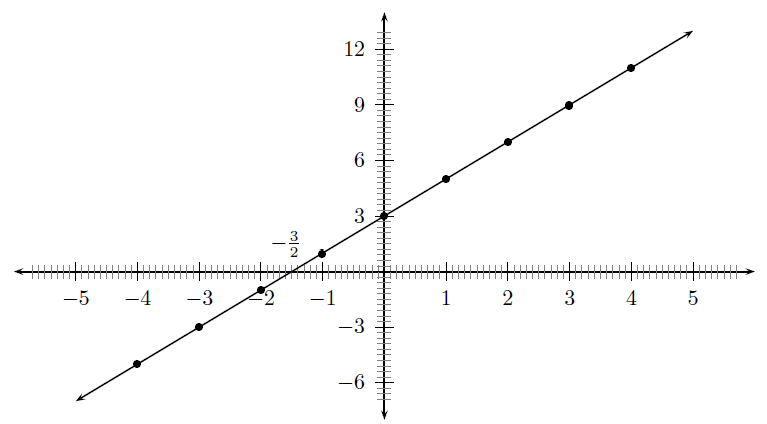
\includegraphics[width=300px]{col11306.imgs/m39338_MG10C11_005.png} % m39338;MG10C11\_005.png;;;6.0;8.5;
      \vspace{2pt}
    \vspace{\rubberspace}\par \begin{cnxcaption}
	  \small \textbf{Figure 1.8: }Graph of $f\left(x\right)=2x+3$
	\end{cnxcaption}
    \vspace{.1in}
    \rule[.1in]{\figurerulewidth}{.005in} \\
    \end{center}
 \end{figure}       
\label{m39338*secfhsst!!!underscore!!!id833}
            \subsection{  Investigating the effects of a and q}
            \nopagebreak
        \label{m39338*id237639}\begin{enumerate}[noitemsep, label=\textbf{\arabic*}. ] 
            \label{m39338*uid70}\item On the same set of axes, plot the following graphs:
\label{m39338*id237654}\begin{enumerate}[noitemsep, label=\textbf{\alph*}. ] 
            \label{m39338*uid71}\item $a\left(x\right)=x-2$\label{m39338*uid72}\item $b\left(x\right)=x-1$\label{m39338*uid73}\item $c\left(x\right)=x$\label{m39338*uid74}\item $d\left(x\right)=x+1$\label{m39338*uid75}\item $e\left(x\right)=x+2$\end{enumerate}
Use your results to deduce the effect of different values of $q$ on the resulting graph.
\label{m39338*uid76}\item On the same set of axes, plot the following graphs:
\label{m39338*id237854}\begin{enumerate}[noitemsep, label=\textbf{\alph*}. ] 
            \label{m39338*uid77}\item $f\left(x\right)=-2\ensuremath{\cdot}x$\label{m39338*uid78}\item $g\left(x\right)=-1\ensuremath{\cdot}x$\label{m39338*uid79}\item $h\left(x\right)=0\ensuremath{\cdot}x$\label{m39338*uid80}\item $j\left(x\right)=1\ensuremath{\cdot}x$\label{m39338*uid81}\item $k\left(x\right)=2\ensuremath{\cdot}x$\end{enumerate}
Use your results to deduce the effect of different values of $a$ on the resulting graph.
\end{enumerate}
        \label{m39338*id238062}You may have noticed that the value of $a$ affects the slope of the graph. As $a$ increases, the slope of the graph increases. If $a\greatthan{}0$ then the graph increases from left to right (slopes upwards). If $a\lessthan{}0$ then the graph increases from right to left (slopes downwards). For this reason, $a$ is referred to as the \textsl{slope} or \textsl{gradient} of a straight-line function.\par 
        \label{m39338*id238136}You should have also found that the value of $q$ affects where the graph passes through the $y$-axis. For this reason, $q$ is known as the \textsl{y-intercept}.\par 
        \label{m39338*id238175}These different properties are summarised in Table 1.7.\par 
    % \textbf{m39338*uid82}\par
          \begin{table}[H]
    % \begin{table}[H]
    % \\ '' '0'
        \begin{center}
      \label{m39345*id240930}
    \noindent
    \tabletail{%
        \hline
        \multicolumn{6}{|p{\mytableboxwidth}|}{\raggedleft \small \sl continued on next page}\\
        \hline
      }
      \tablelasttail{}
      \begin{xtabular}[t]{|l|l|l|l|l|l|}\hline
                  $x$
                 &
                  $-2$
                 &
                  $-1$
                 &
                  $0$
                 &
                  $1$
                 &
                  $2$
                % make-rowspan-placeholders
     \tabularnewline\cline{1-1}\cline{2-2}\cline{3-3}\cline{4-4}\cline{5-5}\cline{6-6}
      %--------------------------------------------------------------------
                  $a\left(x\right)$
                 &
         &
         &
         &
         &
        % make-rowspan-placeholders
     \tabularnewline\cline{1-1}\cline{2-2}\cline{3-3}\cline{4-4}\cline{5-5}\cline{6-6}
      %--------------------------------------------------------------------
                  $b\left(x\right)$
                 &
         &
         &
         &
         &
        % make-rowspan-placeholders
     \tabularnewline\cline{1-1}\cline{2-2}\cline{3-3}\cline{4-4}\cline{5-5}\cline{6-6}
      %--------------------------------------------------------------------
                  $c\left(x\right)$
                 &
         &
         &
         &
         &
        % make-rowspan-placeholders
     \tabularnewline\cline{1-1}\cline{2-2}\cline{3-3}\cline{4-4}\cline{5-5}\cline{6-6}
      %--------------------------------------------------------------------
                  $d\left(x\right)$
                 &
         &
         &
         &
         &
        % make-rowspan-placeholders
     \tabularnewline\cline{1-1}\cline{2-2}\cline{3-3}\cline{4-4}\cline{5-5}\cline{6-6}
      %--------------------------------------------------------------------
                  $e\left(x\right)$
                 &
         &
         &
         &
         &
        % make-rowspan-placeholders
     \tabularnewline\cline{1-1}\cline{2-2}\cline{3-3}\cline{4-4}\cline{5-5}\cline{6-6}
      %--------------------------------------------------------------------
                  $f\left(x\right)$
                 &
         &
         &
         &
         &
        % make-rowspan-placeholders
     \tabularnewline\cline{1-1}\cline{2-2}\cline{3-3}\cline{4-4}\cline{5-5}\cline{6-6}
      %--------------------------------------------------------------------
                  $g\left(x\right)$
                 &
         &
         &
         &
         &
        % make-rowspan-placeholders
     \tabularnewline\cline{1-1}\cline{2-2}\cline{3-3}\cline{4-4}\cline{5-5}\cline{6-6}
      %--------------------------------------------------------------------
                  $h\left(x\right)$
                 &
         &
         &
         &
         &
        % make-rowspan-placeholders
     \tabularnewline\cline{1-1}\cline{2-2}\cline{3-3}\cline{4-4}\cline{5-5}\cline{6-6}
      %--------------------------------------------------------------------
                  $j\left(x\right)$
                 &
         &
         &
         &
         &
        % make-rowspan-placeholders
     \tabularnewline\cline{1-1}\cline{2-2}\cline{3-3}\cline{4-4}\cline{5-5}\cline{6-6}
      %--------------------------------------------------------------------
                  $k\left(x\right)$
                 &
         &
         &
         &
         &
        % make-rowspan-placeholders
     \tabularnewline\cline{1-1}\cline{2-2}\cline{3-3}\cline{4-4}\cline{5-5}\cline{6-6}
      %--------------------------------------------------------------------
    \end{xtabular}
      \end{center}
    \begin{center}{\small\bfseries Table 1.8}\end{center}
    \begin{caption}{\small\bfseries Table 1.8}\end{caption}
\end{table}
    \par
        \label{m39345*eip-679}This simulation allows you to visualise the effect of changing a and q. Note that in this simulation q = c. Also an extra term bx has been added in. You can leave bx as 0, or you can also see what effect this has on the graph.
\par \label{m39345*eip-481}
    \setcounter{subfigure}{0}
	\begin{figure}[H] % horizontal\label{m39345*Ohms-Law}
    \textnormal{Phet simulation for graphing}\vspace{.1in} \nopagebreak
  \label{m39345*phet!!!underscore!!!sim}\label{m39345*phet-simulation}
            \raisebox{-5 pt}{ 
\includegraphics[width=0.5cm]{col11306.imgs/summary_www.png}} { (Simulation:  MG10018 )}
      \vspace{2pt}
    \vspace{.1in}
 \end{figure}       \par \label{m39345*id241684}From your graphs, you should have found that $a$ affects whether the graph makes a smile or a frown. If $a\lessthan{}0$, the graph makes a frown and if $a\greatthan{}0$ then the graph makes a smile. This is shown in Figure~1.18.\par 
    \setcounter{subfigure}{0}
	\begin{figure}[H] % horizontal\label{m39345*uid115}
    \begin{center}
    \rule[.1in]{\figurerulewidth}{.005in} \\
        \label{m39345*uid115!!!underscore!!!media}\label{m39345*uid115!!!underscore!!!printimage}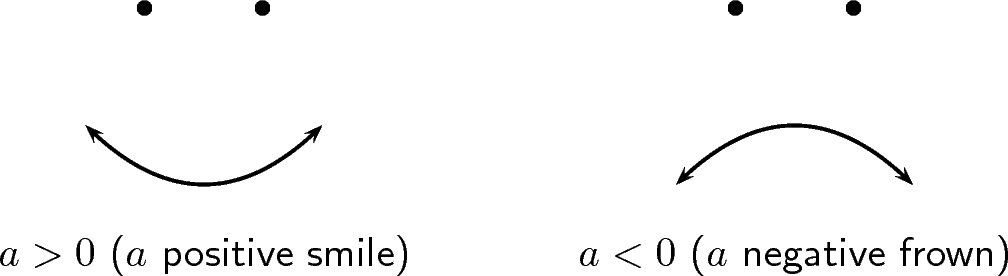
\includegraphics{col11306.imgs/m39345_MG10C11_014.png} % m39345;MG10C11\_014.png;;;6.0;8.5;
      \vspace{2pt}
    \vspace{\rubberspace}\par \begin{cnxcaption}
	  \small \textbf{Figure 1.18: }Distinctive shape of graphs of a parabola if $a\greatthan{}0$ and $a\lessthan{}0$.
	\end{cnxcaption}
    \vspace{.1in}
    \rule[.1in]{\figurerulewidth}{.005in} \\
    \end{center}
 \end{figure}       
        \label{m39345*id241776}You should have also found that the value of $q$ affects whether the turning point is to the left of the $y$-axis ($q\greatthan{}0$) or to the right of the $y$-axis ($q\lessthan{}0$).\par 
        \label{m39345*id241837}These different properties are summarised in Table 1.9.\par 
    % \textbf{m39345*uid116}\par
          \begin{table}[H]
    % \begin{table}[H]
    % \\ '' '0'
        \begin{center}
      \label{m39414*id84073}
    \noindent
    \tabletail{%
        \hline
        \multicolumn{7}{|p{\mytableboxwidth}|}{\raggedleft \small \sl continued on next page}\\
        \hline
      }
      \tablelasttail{}
      \begin{xtabular}[t]{|l|l|l|l|l|l|l|}\hline
                  $\theta $
                 &
                  ${0}^{\circ }$
                 &
                  ${30}^{\circ }$
                 &
                  ${45}^{\circ }$
                 &
                  ${60}^{\circ }$
                 &
                  ${90}^{\circ }$
                 &
                  ${180}^{\circ }$
                % make-rowspan-placeholders
     \tabularnewline\cline{1-1}\cline{2-2}\cline{3-3}\cline{4-4}\cline{5-5}\cline{6-6}\cline{7-7}
      %--------------------------------------------------------------------
                  $sin\theta $
                 &
        0 &
                  $\frac{1}{2}$
                 &
                  $\frac{1}{\sqrt{2}}$
                 &
                  $\frac{\sqrt{3}}{2}$
                 &
        1 &
        0% make-rowspan-placeholders
     \tabularnewline\cline{1-1}\cline{2-2}\cline{3-3}\cline{4-4}\cline{5-5}\cline{6-6}\cline{7-7}
      %--------------------------------------------------------------------
    \end{xtabular}
      \end{center}
    \begin{center}{\small\bfseries Table 14.5}\end{center}
    \begin{caption}{\small\bfseries Table 14.5}\end{caption}
\end{table}
    \par
        \label{m39414*id84327}As you can see, the function $sin\theta $ has a value of 0 at $\theta ={0}^{\circ }$. Its value then smoothly increases until $\theta ={90}^{\circ }$ when its value is 1. We also know that it later decreases to 0 when $\theta ={180}^{\circ }$. Putting all this together we can start to picture the full extent of the sine graph. The sine graph is shown in Figure~14.23. Notice the wave shape, with each wave having a length of ${360}^{\circ }$. We say the graph has a \textsl{period} of ${360}^{\circ }$. The height of the wave above (or below) the $x$-axis is called the wave's \textsl{amplitude}. Thus the maximum amplitude of the sine-wave is 1, and its minimum amplitude is -1.\par 
    \setcounter{subfigure}{0}
	\begin{figure}[H] % horizontal\label{m39414*uid31}
    \begin{center}
    \rule[.1in]{\figurerulewidth}{.005in} \\
        \label{m39414*uid31!!!underscore!!!media}\label{m39414*uid31!!!underscore!!!printimage}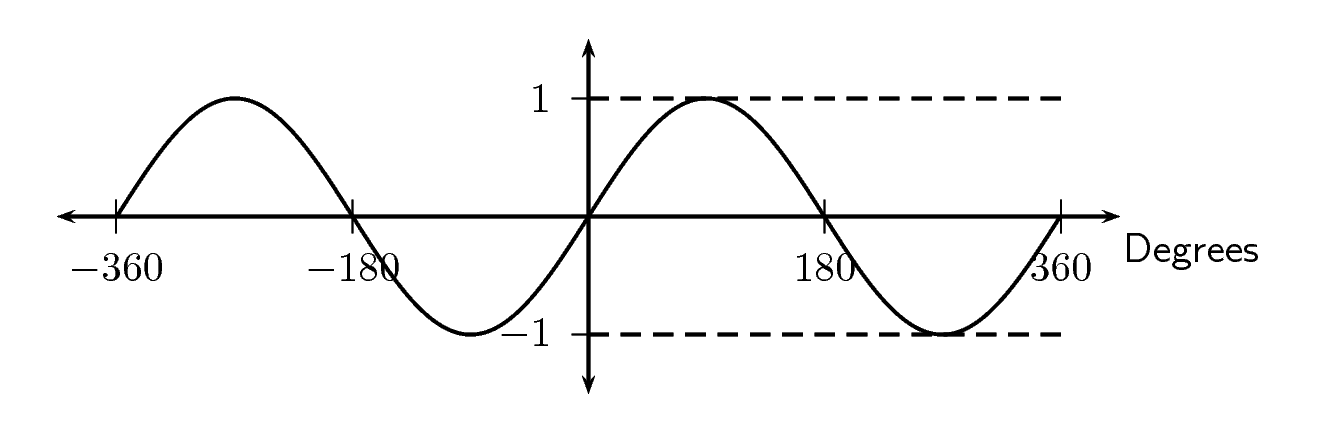
\includegraphics{col11306.imgs/m39414_MG10C15_017.png} % m39414;MG10C15\_017.png;;;6.0;8.5;
      \vspace{2pt}
    \vspace{\rubberspace}\par \begin{cnxcaption}
	  \small \textbf{Figure 14.23: }The graph of $sin\theta $.
	\end{cnxcaption}
    \vspace{.1in}
    \rule[.1in]{\figurerulewidth}{.005in} \\
    \end{center}
 \end{figure}       
      \label{m39414*uid32}
            \subsubsection{ Functions of the form $y=asin\left(x\right)+q$}
            \nopagebreak
        \label{m39414*id84527}In the equation, $y=asin\left(x\right)+q$, $a$ and $q$ are constants and have different effects on the graph of the function. The general shape of the graph of functions of this form is shown in Figure~14.24 for the function $f\left(\theta \right)=2sin\theta +3$.\par 
    \setcounter{subfigure}{0}
	\begin{figure}[H] % horizontal\label{m39414*uid33}
    \begin{center}
    \rule[.1in]{\figurerulewidth}{.005in} \\
        \label{m39414*uid33!!!underscore!!!media}\label{m39414*uid33!!!underscore!!!printimage}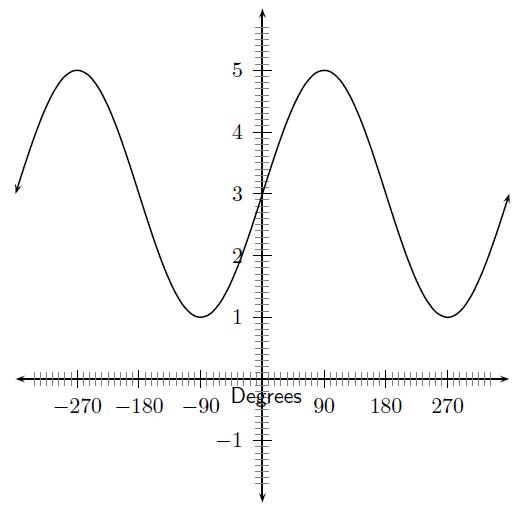
\includegraphics[width=300px]{col11306.imgs/m39414_trigrep.png} % m39414;trigrep.png;;;6.0;8.5;
      \vspace{2pt}
    \vspace{\rubberspace}\par \begin{cnxcaption}
	  \small \textbf{Figure 14.24: }Graph of $f\left(\theta \right)=2sin\theta +3$
	\end{cnxcaption}
    \vspace{.1in}
    \rule[.1in]{\figurerulewidth}{.005in} \\
    \end{center}
 \end{figure}       
\label{m39414*secfhsst!!!underscore!!!id2083}
            \subsubsection{  Functions of the Form $y=asin\left(\theta \right)+q$ :}
            \nopagebreak
        \label{m39414*id84695}\begin{enumerate}[noitemsep, label=\textbf{\arabic*}. ] 
            \label{m39414*uid34}\item On the same set of axes, plot the following graphs:
\label{m39414*id84710}\begin{enumerate}[noitemsep, label=\textbf{\alph*}. ] 
            \label{m39414*uid35}\item $a\left(\theta \right)=sin\theta -2$\label{m39414*uid36}\item $b\left(\theta \right)=sin\theta -1$\label{m39414*uid37}\item $c\left(\theta \right)=sin\theta $\label{m39414*uid38}\item $d\left(\theta \right)=sin\theta +1$\label{m39414*uid39}\item $e\left(\theta \right)=sin\theta +2$\end{enumerate}
Use your results to deduce the effect of $q$.
\label{m39414*uid40}\item On the same set of axes, plot the following graphs:
\label{m39414*id84931}\begin{enumerate}[noitemsep, label=\textbf{\alph*}. ] 
            \label{m39414*uid41}\item $f\left(\theta \right)=-2\ensuremath{\cdot}sin\theta $\label{m39414*uid42}\item $g\left(\theta \right)=-1\ensuremath{\cdot}sin\theta $\label{m39414*uid43}\item $h\left(\theta \right)=0\ensuremath{\cdot}sin\theta $\label{m39414*uid44}\item $j\left(\theta \right)=1\ensuremath{\cdot}sin\theta $\label{m39414*uid45}\item $k\left(\theta \right)=2\ensuremath{\cdot}sin\theta $\end{enumerate}
Use your results to deduce the effect of $a$.
\end{enumerate}
        \label{m39414*id85165}You should have found that the value of $a$ affects the height of the peaks of the graph. As the magnitude of $a$ increases, the peaks get higher. As it decreases, the peaks get lower.\par 
        \label{m39414*id85188}$q$ is called the \textsl{vertical shift}. If $q=2$, then the whole sine graph shifts up 2 units. If $q=-1$, the whole sine graph shifts down 1 unit.\par 
        \label{m39414*id85237}These different properties are summarised in Table 14.6.\par 
    % \textbf{m39414*uid46}\par
          \begin{table}[H]
    % \begin{table}[H]
    % \\ '' '0'
        \begin{center}
      \label{m39414*id86909}
    \noindent
    \tabletail{%
        \hline
        \multicolumn{7}{|p{\mytableboxwidth}|}{\raggedleft \small \sl continued on next page}\\
        \hline
      }
      \tablelasttail{}
      \begin{xtabular}[t]{|l|l|l|l|l|l|l|}\hline
                  $\theta $
                 &
                  ${0}^{\circ }$
                 &
                  ${30}^{\circ }$
                 &
                  ${45}^{\circ }$
                 &
                  ${60}^{\circ }$
                 &
                  ${90}^{\circ }$
                 &
                  ${180}^{\circ }$
                % make-rowspan-placeholders
     \tabularnewline\cline{1-1}\cline{2-2}\cline{3-3}\cline{4-4}\cline{5-5}\cline{6-6}\cline{7-7}
      %--------------------------------------------------------------------
                  $cos\theta $
                 &
        1 &
                  $\frac{\sqrt{3}}{2}$
                 &
                  $\frac{1}{\sqrt{2}}$
                 &
                  $\frac{1}{2}$
                 &
        0 &
                  $-1$
                % make-rowspan-placeholders
     \tabularnewline\cline{1-1}\cline{2-2}\cline{3-3}\cline{4-4}\cline{5-5}\cline{6-6}\cline{7-7}
      %--------------------------------------------------------------------
    \end{xtabular}
      \end{center}
    \begin{center}{\small\bfseries Table 14.8}\end{center}
    \begin{caption}{\small\bfseries Table 14.8}\end{caption}
\end{table}
    \par
        \label{m39414*id87173}If you look carefully, you will notice that the cosine of an angle $\theta $ is the same as the sine of the angle ${90}^{\circ }-\theta $. Take for example,\par 
        \label{m39414*id87206}\nopagebreak\noindent{}
          
    \begin{equation}
    cos{60}^{\circ }=\frac{1}{2}=sin{30}^{\circ }=sin\left({90}^{\circ }-{60}^{\circ }\right)\tag{14.33}
      \end{equation}
        \label{m39414*id87280}This tells us that in order to create the cosine graph, all we need to do is to shift the sine graph ${90}^{\circ }$ to the left. The graph of $cos\theta $ is shown in Figure~14.30. As the cosine graph is simply a shifted sine graph, it will have the same period and amplitude as the sine graph.\par 
    \setcounter{subfigure}{0}
	\begin{figure}[H] % horizontal\label{m39414*uid50}
    \begin{center}
    \rule[.1in]{\figurerulewidth}{.005in} \\
        \label{m39414*uid50!!!underscore!!!media}\label{m39414*uid50!!!underscore!!!printimage}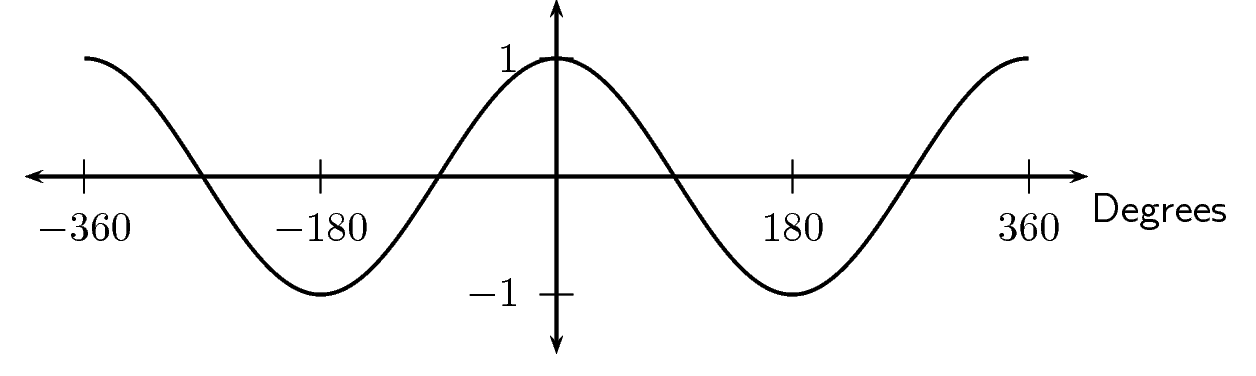
\includegraphics{col11306.imgs/m39414_MG10C15_024.png} % m39414;MG10C15\_024.png;;;6.0;8.5;
      \vspace{2pt}
    \vspace{\rubberspace}\par \begin{cnxcaption}
	  \small \textbf{Figure 14.30: }The graph of $cos\theta $.
	\end{cnxcaption}
    \vspace{.1in}
    \rule[.1in]{\figurerulewidth}{.005in} \\
    \end{center}
 \end{figure}       
      \label{m39414*uid51}
            \subsubsection{ Functions of the form $y=acos\left(x\right)+q$}
            \nopagebreak
        \label{m39414*id87386}In the equation, $y=acos\left(x\right)+q$, $a$ and $q$ are constants and have different effects on the graph of the function. The general shape of the graph of functions of this form is shown in Figure~14.31 for the function $f\left(\theta \right)=2cos\theta +3$.\par 
    \setcounter{subfigure}{0}
	\begin{figure}[H] % horizontal\label{m39414*uid52}
    \begin{center}
    \rule[.1in]{\figurerulewidth}{.005in} \\
        \label{m39414*uid52!!!underscore!!!media}\label{m39414*uid52!!!underscore!!!printimage}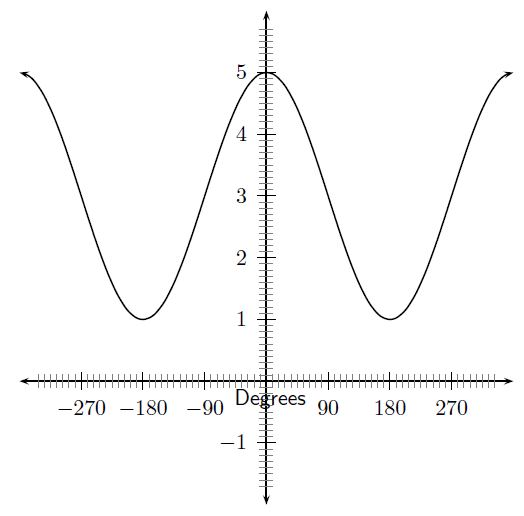
\includegraphics[width=300px]{col11306.imgs/m39414_trigrep1.png} % m39414;trigrep1.png;;;6.0;8.5;
      \vspace{2pt}
    \vspace{\rubberspace}\par \begin{cnxcaption}
	  \small \textbf{Figure 14.31: }Graph of $f\left(\theta \right)=2cos\theta +3$
	\end{cnxcaption}
    \vspace{.1in}
    \rule[.1in]{\figurerulewidth}{.005in} \\
    \end{center}
 \end{figure}       
\label{m39414*secfhsst!!!underscore!!!id2647}
            \subsubsection{  Functions of the Form $y=acos\left(\theta \right)+q$ :}
            \nopagebreak
        \label{m39414*id87553}\begin{enumerate}[noitemsep, label=\textbf{\arabic*}. ] 
            \label{m39414*uid53}\item On the same set of axes, plot the following graphs:
\label{m39414*id87568}\begin{enumerate}[noitemsep, label=\textbf{\alph*}. ] 
            \label{m39414*uid54}\item $a\left(\theta \right)=cos\theta -2$\label{m39414*uid55}\item $b\left(\theta \right)=cos\theta -1$\label{m39414*uid56}\item $c\left(\theta \right)=cos\theta $\label{m39414*uid57}\item $d\left(\theta \right)=cos\theta +1$\label{m39414*uid58}\item $e\left(\theta \right)=cos\theta +2$\end{enumerate}
Use your results to deduce the effect of $q$.
\label{m39414*uid59}\item On the same set of axes, plot the following graphs:
\label{m39414*id87790}\begin{enumerate}[noitemsep, label=\textbf{\alph*}. ] 
            \label{m39414*uid60}\item $f\left(\theta \right)=-2\ensuremath{\cdot}cos\theta $\label{m39414*uid61}\item $g\left(\theta \right)=-1\ensuremath{\cdot}cos\theta $\label{m39414*uid62}\item $h\left(\theta \right)=0\ensuremath{\cdot}cos\theta $\label{m39414*uid63}\item $j\left(\theta \right)=1\ensuremath{\cdot}cos\theta $\label{m39414*uid64}\item $k\left(\theta \right)=2\ensuremath{\cdot}cos\theta $\end{enumerate}
Use your results to deduce the effect of $a$.
\end{enumerate}
        \label{m39414*id88024}You should have found that the value of $a$ affects the amplitude of the cosine graph in the same way it did for the sine graph.\par 
        \label{m39414*id88038}You should have also found that the value of $q$ shifts the cosine graph in the same way as it did the sine graph.\par 
        \label{m39414*id88050}These different properties are summarised in Table 14.9.\par 
    % \textbf{m39414*uid65}\par
          \begin{table}[H]
    % \begin{table}[H]
    % \\ '' '0'
        \begin{center}
      \label{m39414*id89593}
    \noindent
    \tabletail{%
        \hline
        \multicolumn{7}{|p{\mytableboxwidth}|}{\raggedleft \small \sl continued on next page}\\
        \hline
      }
      \tablelasttail{}
      \begin{xtabular}[t]{|l|l|l|l|l|l|l|}\hline
                  $\theta $
                 &
                  ${0}^{\circ }$
                 &
                  ${30}^{\circ }$
                 &
                  ${45}^{\circ }$
                 &
                  ${60}^{\circ }$
                 &
                  ${90}^{\circ }$
                 &
                  ${180}^{\circ }$
                % make-rowspan-placeholders
     \tabularnewline\cline{1-1}\cline{2-2}\cline{3-3}\cline{4-4}\cline{5-5}\cline{6-6}\cline{7-7}
      %--------------------------------------------------------------------
                  $tan\theta $
                 &
        0 &
                  $\frac{1}{\sqrt{3}}$
                 &
        1 &
                  $\sqrt{3}$
                 &
                  $\infty $
                 &
        0% make-rowspan-placeholders
     \tabularnewline\cline{1-1}\cline{2-2}\cline{3-3}\cline{4-4}\cline{5-5}\cline{6-6}\cline{7-7}
      %--------------------------------------------------------------------
    \end{xtabular}
      \end{center}
    \begin{center}{\small\bfseries Table 14.11}\end{center}
    \begin{caption}{\small\bfseries Table 14.11}\end{caption}
\end{table}
    \par
        \label{m39414*id89839}Now that we have graphs for $sin\theta $ and $cos\theta $, there is an easy way to visualise the tangent graph. Let us look back at our definitions of $sin\theta $ and $cos\theta $ for a right-angled triangle.\par 
        \label{m39414*id89902}\nopagebreak\noindent{}
          
    \begin{equation}
    \frac{sin\theta }{cos\theta }=\frac{\frac{\mathrm{opposite}}{\mathrm{hypotenuse}}}{\frac{\mathrm{adjacent}}{\mathrm{hypotenuse}}}=\frac{\mathrm{opposite}}{\mathrm{adjacent}}=tan\theta \tag{14.36}
      \end{equation}
        \label{m39414*id89965}This is the first of an important set of equations called \textsl{trigonometric identities}. An identity is an equation, which holds true for any value which is put into it. In this case we have shown that\par 
        \label{m39414*id89978}\nopagebreak\noindent{}
          
    \begin{equation}
    tan\theta =\frac{sin\theta }{cos\theta }\tag{14.37}
      \end{equation}
        \label{m39414*id90014}for any value of $\theta $.\par 
        \label{m39414*id90030}So we know that for values of $\theta $ for which $sin\theta =0$, we must also have $tan\theta =0$. Also, if $cos\theta =0$ our value of $tan\theta $ is undefined as we cannot divide by 0. The graph is shown in Figure~14.38. The dashed vertical lines are at the values of $\theta $ where $tan\theta $ is not defined.\par 
    \setcounter{subfigure}{0}
	\begin{figure}[H] % horizontal\label{m39414*uid71}
    \begin{center}
    \rule[.1in]{\figurerulewidth}{.005in} \\
        \label{m39414*uid71!!!underscore!!!media}\label{m39414*uid71!!!underscore!!!printimage}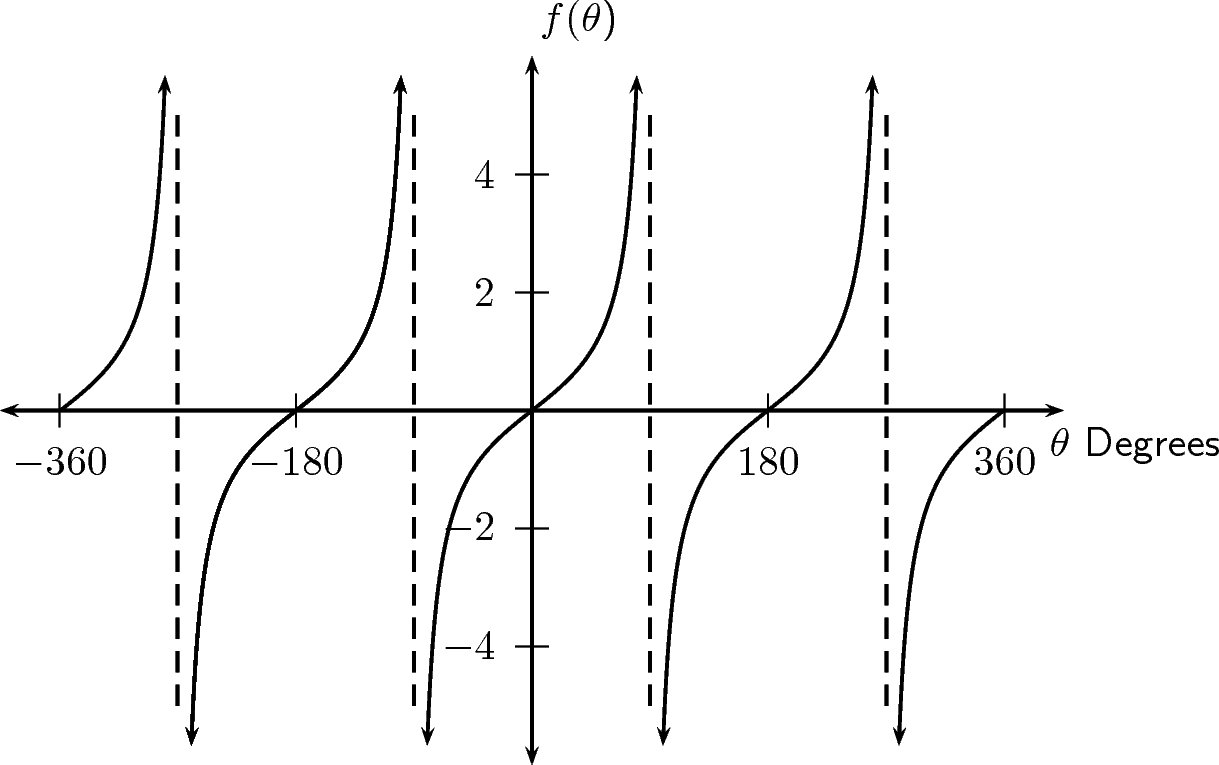
\includegraphics{col11306.imgs/m39414_MG10C15_044.png} % m39414;MG10C15\_044.png;;;6.0;8.5;
      \vspace{2pt}
    \vspace{\rubberspace}\par \begin{cnxcaption}
	  \small \textbf{Figure 14.38: }The graph of $tan\theta $.
	\end{cnxcaption}
    \vspace{.1in}
    \rule[.1in]{\figurerulewidth}{.005in} \\
    \end{center}
 \end{figure}       
      \label{m39414*uid72}
            \subsubsection{ Functions of the form $y=atan\left(x\right)+q$}
            \nopagebreak
        \label{m39414*id90209}In the figure below is an example of a function of the form $y=atan\left(x\right)+q$.\par 
    \setcounter{subfigure}{0}
	\begin{figure}[H] % horizontal\label{m39414*uid73}
    \begin{center}
    \rule[.1in]{\figurerulewidth}{.005in} \\
        \label{m39414*uid73!!!underscore!!!media}\label{m39414*uid73!!!underscore!!!printimage}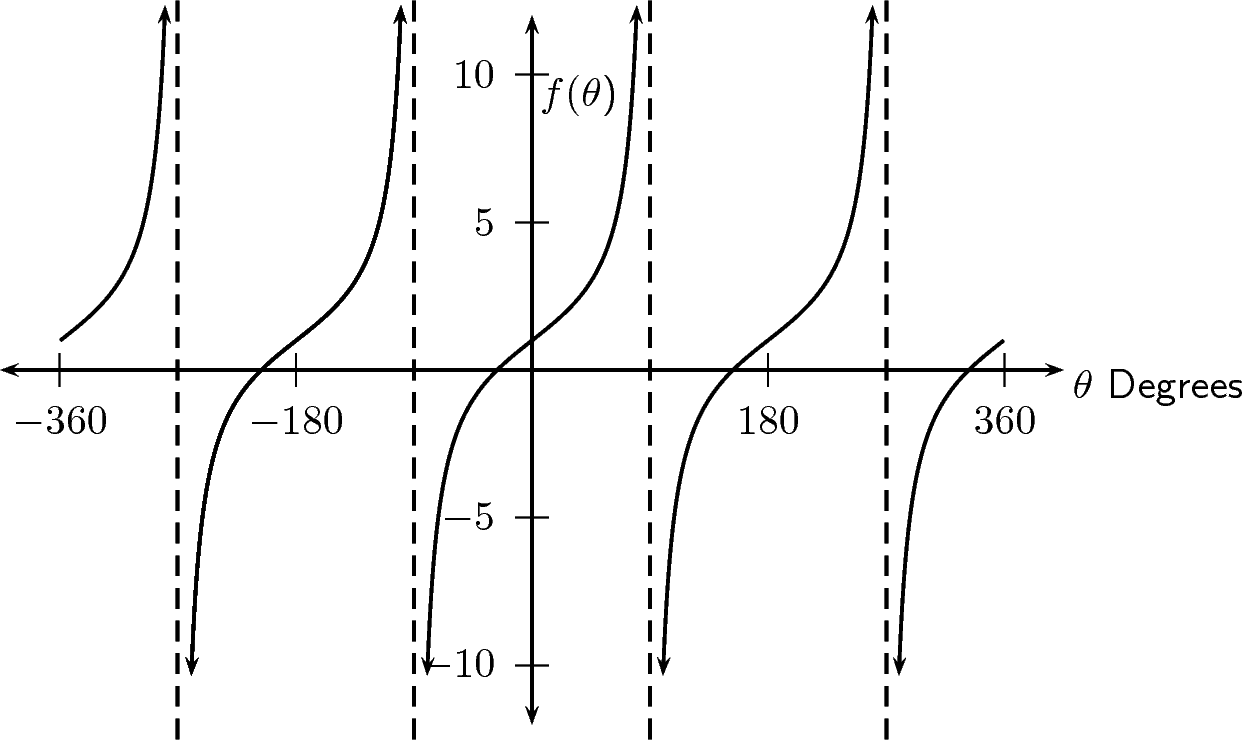
\includegraphics{col11306.imgs/m39414_MG10C15_045.png} % m39414;MG10C15\_045.png;;;6.0;8.5;
      \vspace{2pt}
    \vspace{\rubberspace}\par \begin{cnxcaption}
	  \small \textbf{Figure 14.39: }The graph of $2tan\theta +1$.
	\end{cnxcaption}
    \vspace{.1in}
    \rule[.1in]{\figurerulewidth}{.005in} \\
    \end{center}
 \end{figure}       
\label{m39414*secfhsst!!!underscore!!!id3205}
            \subsubsection{  Functions of the Form $y=atan\left(\theta \right)+q$ :}
            \nopagebreak
        \label{m39414*id90310}\begin{enumerate}[noitemsep, label=\textbf{\arabic*}. ] 
            \label{m39414*uid74}\item On the same set of axes, plot the following graphs:
\label{m39414*id90326}\begin{enumerate}[noitemsep, label=\textbf{\alph*}. ] 
            \label{m39414*uid75}\item $a\left(\theta \right)=tan\theta -2$\label{m39414*uid76}\item $b\left(\theta \right)=tan\theta -1$\label{m39414*uid77}\item $c\left(\theta \right)=tan\theta $\label{m39414*uid78}\item $d\left(\theta \right)=tan\theta +1$\label{m39414*uid79}\item $e\left(\theta \right)=tan\theta +2$\end{enumerate}
Use your results to deduce the effect of $q$.
\label{m39414*uid80}\item On the same set of axes, plot the following graphs:
\label{m39414*id90547}\begin{enumerate}[noitemsep, label=\textbf{\alph*}. ] 
            \label{m39414*uid81}\item $f\left(\theta \right)=-2\ensuremath{\cdot}tan\theta $\label{m39414*uid82}\item $g\left(\theta \right)=-1\ensuremath{\cdot}tan\theta $\label{m39414*uid83}\item $h\left(\theta \right)=0\ensuremath{\cdot}tan\theta $\label{m39414*uid84}\item $j\left(\theta \right)=1\ensuremath{\cdot}tan\theta $\label{m39414*uid85}\item $k\left(\theta \right)=2\ensuremath{\cdot}tan\theta $\end{enumerate}
Use your results to deduce the effect of $a$.
\end{enumerate}
        \label{m39414*id90781}You should have found that the value of $a$ affects the steepness of each of the branches. The larger the absolute magnitude of \textsl{a}, the quicker the branches approach their asymptotes, the values where they are not defined. Negative $\mathit{a}$ values switch the direction of the branches.
You should have also found that the value of $q$ affects the vertical shift as for $sin\theta $ and $cos\theta $.
These different properties are summarised in Table 14.12.\par 
    % \textbf{m39414*uid86}\par
